\chapter{Introduction}
\label{cha:introduction}

Today a world without internet is unimaginable to many people. It affects almost all areas of our daily life. In a minute, for example, $3.7$ million search queries are made on Google, $18$ million messages are sent on Whatsapp, and $4.3$ million videos are viewed on YouTube (see \Cref{fig:60minutes}). Furthermore, at the same time many websites are created, blog entries are written, videos and pictures are uploaded and shared. Hence, users generate a lot of data. Due to this vast amount of generated data, almost everything can be found on the internet.

\myfig{60minutes}
      {width=0.62\textwidth}
      {\textbf{User activity of the Internet in 2018.} The Internet has become a daily companion, and is an indispensable part of life. This figure gives an overview of what happens within the most popular services in a single minute. Retrieved July 19, 2019 from \url{https://www.allaccess.com/merge/archive/28030/2018-update-what-happens-in-an-internet-minute}}
      {User activity of the Internet in 2018.}
      {fig:60minutes}

In order to find relevant information, the challenge becomes to filter the data, because a typical user is usually interested in a specific piece of information. Applications which use information retrieval to find relevant information for the user are known as search engines. To be more specific, a search engine helps to reduce the time required to find a piece of information, and minimize the number of information sources that need to be searched. That sounds very simple at first, but each user has different subjective expectations, and therefore search engines have to fulfill different requirements. For example, a user uses a web search engine to search for "restaurant". Normally, the top recommendations would be restaurants near the user, or the best restaurants in town. But on the other hand the user could not be interested in eating, but wants to know the origin of the word.

During a single request search engines leverage different information channels. First, information provided by the user. For many known search engines, these are key words used as a query. Another possibility is to search with files like pictures, articles, or scientific papers. When a search engine uses only this type of information it is called an explicit search. The explicit search process itself works in a way that stored data is examined first. Afterwards the results are ranked according to their relevance. Finally, the user gets an sorted list with the best results on top of the list.

However, there is also other implicit information available, which was not explicitly provided by the user. With this additional information, the results can be better adapted to the needs of the user. For example Agichtein et al. ~\cite{agichtein2006improving} use machine learning approaches to take user actions during the search process into account. Leveraging this type of information in addition to information provided by the user is denoted implicit search.


\section{Motivation}
\label{sec:Motivation}

Search engines are used in many different areas. One of them is in the field of science, where they simplify literature search. Before there were search engines on the Internet, literature search was only possible in libraries. The search was more complicated, since certain literature was only available in certain libraries. This resulted in a time expenditure, since literature had to be sent or picked up. In addition, all publications needed to be examined by the user itself. Overall the search of relevant literature was tedious for the user and a time consuming process.

Modern search engines made searching in the field of science more comfortable. With a single query all publications are searched for the query words. Normally, this takes only a few seconds. The ranking of the results also gives a first overview which literature is relevant for the user. To provide these publications to the user the search results typically contain a link to the publications.

The main goal of our thesis is to apply structural document information of scientific papers into the most common ranking algorithms of search engines. In general, a ranking algorithm ranks based on keywords in the text areas of scientific papers. Therefore, when two papers are related to each other they have similar keywords. We deduce that a more targeted search is possible by providing the information of the section where the keywords are located. For example, if the introduction is compared there is only a subset of keywords where the similarity depends on.

 L.B. Sollaci and M.G. Pereira~\cite{Sollaci-The-2004} describe in their work how the structure of a scientific paper changed over time. They concluded that the subdivision into introduction, method, result, and discussion became a common format in the course of the twentieth century. This subdivision is better known as the IMRaD structure, which we used as a base. This means we created a mapping from the chapter titles to this structure. Additionally, we adapted the ranking algorithms in a way that they take this structural information into account.

 % TODO: Resultate ganz lowlevel

\section{Research Questions}
\label{sec:research_questions}

In general, we tackle the question whether it is possible to improve the search result quality while searching for scientific works by using IMRaD structure information. This means we evaluate if our adapted algorithms can achieve better results with the usage of IMRaD structure information than the standard version.

Hence, the following research questions arise:

\begin{figure}[t]
  \begin{subfigure}[c]{0.49\textwidth}
    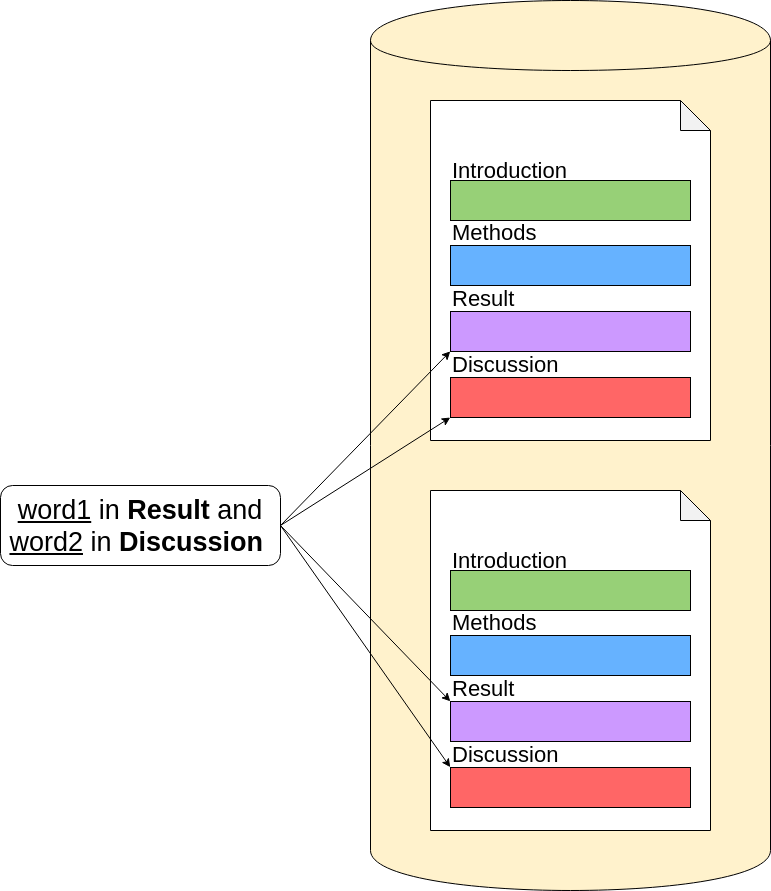
\includegraphics[width=0.9\textwidth]{figures/explicit}
    \subcaption{Explicit Search}
  \end{subfigure}
  \begin{subfigure}[c]{0.49\textwidth}
    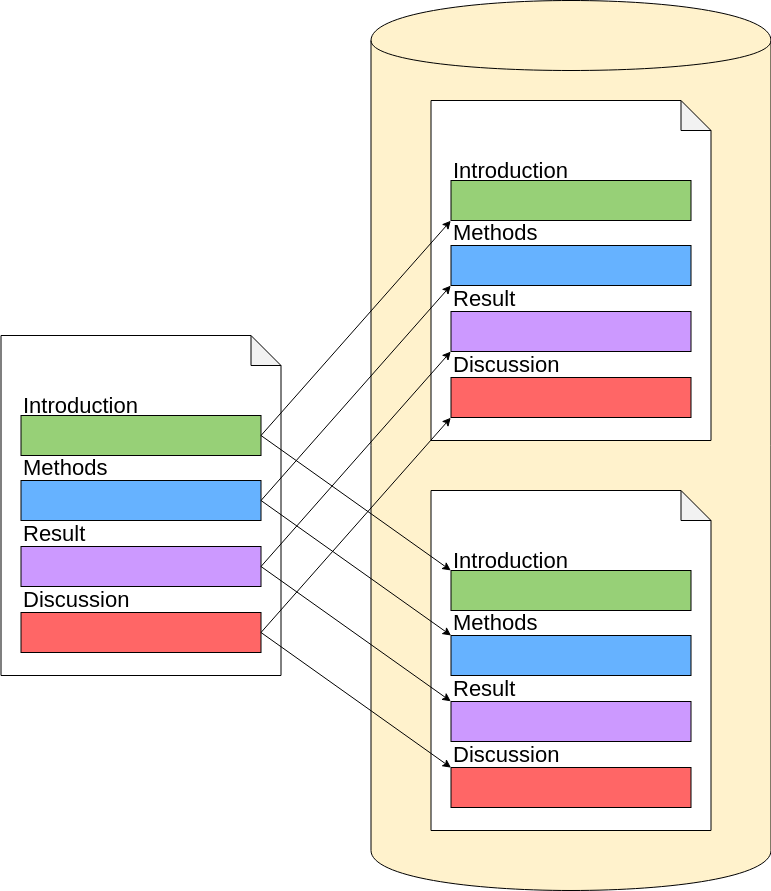
\includegraphics[width=0.9\textwidth]{figures/implicit}
    \subcaption{Implicit Search}
  \end{subfigure}
  \caption[Explicit and Implicit Search using Document Structure Information]{\textbf{Explicit and Implicit Search using Document Structure Information.} Using explicit search (a) the user have to define where query words should occur. Then the specified areas of each scientific work in the database are searched through the word. The difference of implicit search (b) is that the user does not recognize the usage of structural information within the search engine. If a scientific work is used to search for other scientific works the words in the document gets structured by the search engine.}
  \label{fig:implicit_vs_explicit}
\end{figure}

\begin{enumerate}
  \item Does the search result improve for explicit search using queries?
\end{enumerate}

The hypothesis is that used keywords vary in different areas. This leads to the idea that a more targeted search is possible if a user can specify where query words should occur (see \Cref{fig:implicit_vs_explicit} a).

\begin{enumerate}
  \setcounter{enumi}{1}
  \item Does the search result improve for implicit search using complete scientific papers?
\end{enumerate}

When a paper is used as a query, the query words and the structure information are available. Therefore, the query words can be mapped to their occurred chapter. (see \Cref{fig:implicit_vs_explicit} b). Using the same assumption than in the previous question, the similarity of the scientific papers should be higher.

\myfig{input_search_areas}
      {width=0.45\textwidth}
      {\textbf{Difference between Input Areas and Search Areas.} When using a scientific work to search implicit for other scientific works there are two different areas. The first is the input area which is part of the used scientific work. The second one is the search area where query words of the input area should occur. The used chapters of the input area do not have to be the same as the chapters of the search area.}
      {Difference between Input Areas and Search Areas}
      {fig:input_search_areas}

\begin{enumerate}
  \setcounter{enumi}{2}
  \item Does the search result improve if only a single chapter of the scientific paper is used for searching?
\end{enumerate}

The hypothesis is that each chapter has a different influence on the search result. Therefore, there are chapters with a higher impact than others, which could be positive for the resulting list, but also be negative. The idea is to improve the result by using only chapters with a positive effect.

Furthermore, keywords of a chapter can be used in other chapters (see \Cref{fig:input_search_areas}). For example, the Methods section of one paper would be referenced in the Related Work of another paper.
